\selectlanguage{german}
\thispagestyle{empty}
{\vrule height 0mm depth 30mm width 0mm}
%\vspace*{2em}
\par\noindent 
\uppercase{Textgestaltung}\par\vspace{1.0ex}
\noindent Bei der Textgestaltung werden die Grunds\"{a}tze befolgt, die in den Vorworten zu den B\"{a}nden I,5 und VI,6 als f\"{u}r alle Reihen verbindlich festgelegt wurden. Dabei gilt insbesondere:\par
1. Jedes unbetitelte St\"{u}ck erh\"{a}lt eine \"{U}berschrift in der Sprache des St\"{u}ckes. Eigene \"{U}berschriften von Leibniz werden \"{u}bernommen, jedoch hinsichtlich der Gro{\ss}- und Kleinschreibung sowie der Akzentuierungen den anderen \"{U}berschriften angepasst. Das Leibniz'sche Original wird unmittelbar vor dem Text wiederholt.\par
2. Die Gro{\ss}- und Kleinschreibung lateinischer Texte wird gem\"{a}{\ss} den Editionen der Klassiker normalisiert. Insbesondere werden i und j sowie u und v entsprechend vereinheitlicht. Vollst\"{a}ndige S\"{a}tze werden mit einem Punkt abgeschlossen. Jeder Satzanfang wird gro{\ss} geschrieben. Akzente fallen weg.\par
3. In franz\"{o}sischen Texten wird das Schriftbild beibehalten, jedoch werden Akzente dort erg\"{a}nzt, wo Missverst\"{a}ndnisse entstehen k\"{o}nnen. Fehlt bei Leibniz offensichtlich ein Apostroph, so erg\"{a}nzen wir es. Wenn ein \glqq que`` als K\"{u}rzel auftritt, wird es im modernen Sinne aufgel\"{o}st. Sprachliche Versehen werden verbessert, wenn Leibniz die richtige Form zur fraglichen Zeit kennt und verwendet (Beispiel: certaines corps \textit{L} statt certains corps wird verbessert). Sie werden beibehalten, wenn Leibniz die falsche Form vors\"{a}tzlich, etwa auf Grund einer \"{A}nderung, niederschreibt (Beispiel: contante), seine Kenntnis der richtigen Form also nicht sicher belegt ist.\par
4. Die Leibniz'sche Interpunktion wird bewahrt. Hinzugef\"{u}gte Zeichen werden, abgesehen von den unter Punkt 2 und 3 genannten F\"{a}llen sowie bei offensichtlichen Fl\"{u}chtigkeiten, in eckige Klammern gesetzt.\par
\par\vspace{5.0ex}
%\clearpage
\noindent\uppercase{Variantengestaltung}\par\vspace{1.0ex}
\noindent
Die Variantengestaltung erfolgt gem\"{a}{\ss} den Regeln der anderen Reihen. Eine Variante ist durch Zeilenangabe sowie vorderen und hinteren Anschluss eindeutig mit dem Haupttext verkn\"{u}pft. Streichungen werden zwischen senkrechte Striche gesetzt, Erg\"{a}nzungen durch blo{\ss}e Angabe des hinzugef\"{u}gten Textes dargestellt. Bei Ersetzungen kennzeichnen vorangestellte Ziffern \textit{(1)}, \textit{(2)}, \textit{(3)} ... und Buchstaben \textit{(a)}, \textit{(b)}, \textit{(c)} ..., \textit{(aa)}, \textit{(bb)}, \textit{(cc)} ... die Stufen der Gedankenentwicklung. Jede nachfolgende Stufe hebt die vorhergehende auf. Nachgestellte Siglen (in diesem Band meist \textit{L}) bezeichnen den Textzeugen, welchem die Variante entnommen ist. Um bei tief gestuften Varianten die \"{U}bersicht zu wahren, werden die Bezeichnungen zu F\"{u}nfergruppen zusammengefasst und wie folgt wiedergegeben: \textit{(aaaaa-a)} ... \textit{(bbbbb-b)} ... \textit{(aaaaa-aa)} ... \textit{(bbbbb-bb)} usw. Treten innerhalb von Varianten Erg\"{a}nzungen und Streichungen auf, die ihrerseits wieder Varianten enthalten, so werden solche Streichungen und Erg\"{a}nzungen als eigenst\"{a}ndige Textteile behandelt. Die Variantenz\"{a}hlung beginnt in diesen F\"{a}llen neu.\par
In den Varianten werden Wortlaut, Zeichensetzung und Rechnungen grunds\"{a}tzlich nicht berichtigt, auch nicht bei offensichtlichen Fehlern. Abbrechende W\"{o}rter werden nicht vervollst\"{a}ndigt. Die letzte Korrekturstufe wird nur abgek\"{u}rzt wiedergegeben. Die Auslassungen werden durch Punkte in eckigen Klammern kenntlich gemacht.\par\vspace{2.0ex}
%\clearpage
\noindent Beispieltext zur Variantengestaltung aus VIII,1 N.~21\raisebox{-0.5ex}{\notsotiny2}\par\vspace{1.0ex}
\noindent21\hspace{1cm}[...] decurrat. Sed quam precaria quantisque difficultatibus\\
22\hspace{1cm}obsita sit haec Hypothesis quam aliena similitudine confirmata dudum a\\ multis observatum\\
23\hspace{1cm}est.\par\vspace{0.5cm}
\noindent \footnotesize 21\textendash 23 decurrat. \textit{(1)} Sed \textit{(a)} quam obscura \textit{(b)} quam obnoxia difficultatibus \textit{(c)} quis concedat \textit{(aa)} omne rar \textit{(bb)} quantum unum quodque corpus est, rarius tanto esse villo. \textit{(2)} Sed \textit{(a)} quantis difficultati \textit{(b)} quam [...] Hypothesis \textbar\ quam aliena similitudine \textit{(1)} adhibita \textit{(2)} confirmata; dudum \textit{erg.}\ \textbar\ a multis \textit{(aa)} expositum est \textit{(aaa)} vero \textit{(bbb)} et ausim dicere vix \textit{(bb)} observatum est. \textit{L}\par
%\vspace{1.0ex}
\noindent 21\textendash 23 decurrat.\par\noindent
\hspace{3mm}\textit{(1)}\ Sed\par\noindent
\hspace{8mm}\textit{(a)}\ quam obscura\par\noindent
\hspace{8mm}\textit{(b)}\ quam obnoxia difficultatibus\par\noindent
\hspace{8mm}\textit{(c)}\ quis concedat\par\noindent
\hspace{18mm}\textit{(aa)}\ omne rar\par\noindent
\hspace{18mm}\textit{(bb)}\ quantum unum quodque corpus est, rarius tanto esse villo.\par\noindent
\hspace{3mm}\textit{(2)}\ Sed\par\noindent
\hspace{8mm}\textit{(a)}\ quantis difficultati\par\noindent
\hspace{8mm}\textit{(b)}\ quam [...] Hypothesis \textbar\ quam aliena similitudine \textit{(1)} adhibita\par\noindent
\hspace{8.3cm}\textit{(2)}\ confirmata; dudum \textit{erg.} \textbar\ a
multis\par\noindent
\hspace{18mm}\textit{(aa)}\ expositum est\par\noindent
\hspace{23mm}\textit{(aaa)} vero\par\noindent
\hspace{23mm}\textit{(bbb)} et ausim dicere vix\par\noindent
\hspace{18mm}\textit{(bb)} observatum est. \textit{L}
\par\vspace{5.0ex}
\normalsize
%\clearpage
\noindent\uppercase{Rechnungen und Notation}\par\vspace{1.0ex}
\noindent Die Leibniz'sche mathematische Notation wird durch Kursivierung verein\-heitlicht. Nebenrechnungen werden wie Marginalien behandelt und direkt unter den Text gesetzt. Leibniz benutzt die zu seiner Zeit \"{u}bliche \"{U}berw\"{a}rtsdivision mit ihren charakteristischen Streichungen und rechnet gelegentlich \glqq fortlaufend`` weiter, d. h. er verwendet bei Gleichungsketten Zwischenergebnisse ohne Neuansatz (vgl. VIII,1 N.~36).\par
%\vspace{-0.2mm}
\begin{center}
$\begin{array}{lllr}             
\hspace{5.5pt}\cancel{3}2&&&\\
\hspace{5.5pt}\cancel{7}\cancel{8}&&&\\
\cancel{2}\cancel{3}\cancel{6}2&&\hspace{11pt}2644&\\
\cancel{7}\cancel{2}\cancel{2}\cancel{5}&f&\hspace{16.5pt}147&\\
\cancel{4}\cancel{9}\cancel{9}\cancel{9}&&\overline{\hspace{5.5pt}18508}&\\
\hspace{5.5pt}\cancel{4}\cancel{4}&&10576&\\
  &&2644&\\
  &&\overline{388668}&
 \end{array}$  
\end{center}
Zu den Besonderheiten der Rechentechnik geh\"{o}rt weiterhin, dass Leibniz zur Vermeidung von Fallunterscheidungen Doppelvorzeichen verwendet, die paarweise oder auch mehrfach zusammengesetzt sein können. Dar\"{u}ber hinaus benutzt er neben den auch heute \"{u}blichen runden Klammern ein- bzw. zweiseitige Halbklammern, die im Text durch Kommata bzw. $\llcorner$  und $\lrcorner$ wiedergegeben werden (vgl. N.~54).\par
%  \def\leibdashvv{\diatop[$\vspace{10pt}-$|$|$]}
%                     \def\leibdashv{\diatop[$\leibdashvv$|$\hspace{-5.15pt}\dashv$]}
%                    \def\leibvdash{\protect\raisebox{10.5pt}{\protect\scalebox{1}[-1]{$\leibdashv$}}}      
                    \begin{center}
$\protect\begin{array}{rl}\displaystyle \leibdashv \hspace{5pt} x \hspace{5pt} \leibvdash \hspace{5pt} \displaystyle\protect\frac{\beta^2}{2} &\protect\sqcap\hspace{5pt} \protect\sqrt{ \protect\llcorner \displaystyle\protect\frac{1}{4} - 2 \protect\lrcorner \beta^2,, + \protect\llcorner 4 - \displaystyle\protect\frac{1}{2}a \protect\lrcorner \displaystyle\protect\frac{a^3\beta}{n^2},, + \protect\llcorner8 - \displaystyle\protect\frac{1}{8}\protect\lrcorner \protect\frac{a^6}{n^4}}\vspace{0.1cm}\\ \displaystyle\protect\frac{4a^3}{n^2}&\protect\end{array}$
\end{center}
Aus Gr\"{u}nden der Vereinfachung von Gleichungen und Termen markiert Leibniz einzelne Rechenschritte durch Streichungen oder abgerundete Umrahmungen, und er bezeichnet in mehrzeiligen Schemata mehrfach auftretende Formelbestandteile durch Punktierung (vgl. N.~54).
\begin{center}
   $\begin{array}{r}\displaystyle z^4- 8ax\hspace{3pt}z^2\\+4a\beta ..\\\rule[0cm]{0cm}{20pt}
                               \end{array}
                               \Bigg\{\begin{array}{ll}\displaystyle+64a^2x^2&\sqcap\\\displaystyle-64a^2\beta x&\\\displaystyle \frac{+16a^2\beta^2}{4}&\end{array}
                     \begin{array}{ll}\displaystyle+8a^2x^2&\\\displaystyle-8a^2\beta x&\\\displaystyle \ovalbox{$+4a^2\beta^2\hspace{-35pt}\raisebox{-13pt}{$-4a^2\beta^2$}$}&\end{array}$
\end{center}
\newpage
\par
\par\vspace{5.0ex}
\noindent\uppercase{Besonderheiten bei Figuren und Zeichnungen}\par\vspace{1.0ex}
\noindent
Figuren und Zeichnungen wurden von Leibniz in der Regel in Tinte aus\-gef\"{u}hrt. Nicht ungew\"{o}hnlich sind auch Zeichnungen, die teilweise als Blind\-zeichnungen \"{u}berliefert sind. Seltener treten Bleistiftzeichnungen auf. Die Blind\-zeichnungen werden von den \"{u}brigen durch Aufhellung unterschieden. Sie erscheinen daher im Druckbild grau.\par
S\"{a}mtliche Figuren und Zeichnungen werden f\"{u}r den Fall, dass Leibniz sie nicht bezeichnet hat, st\"{u}ckbezogen durchnummeriert. Die vom Editor hinzugef\"{u}gten Bezeichnungen werden in eckige Klammern gesetzt und kursiviert.\par
Die Notation innerhalb von Zeichnungen wird mit der des Schriftbefunds abgeglichen und kursiv wiedergegeben. Dabei werden Gro{\ss}- und Kleinschreibung harmonisiert. Fehlende Notationen innerhalb von Zeichnungen werden in eckigen Klammern hinzugef\"{u}gt. \par
Die Figuren und Zeichnungen aus den Marginalienexemplaren wurden dem Original folgend nachgezeichnet. Dadurch kann es zu Abweichungen in der Strich\-st\"{a}rke sowie hinsichtlich der Kursivierung der Bezeichnungen kommen. In diesen Exemplaren hat Leibniz h\"{a}ufig Elemente von Zeichnungen durch Zus\"{a}tze versehen. F\"{u}r den Fall, dass es sich dabei um Bezeichnungen handelt, werden diese Zus\"{a}tze durch runde kursivierte Klammern kenntlich gemacht.
%\clearpage
Beispiel einer Zeichnung mit Blindzeichnung und nachtr\"{a}glich vom Editor hinzugef\"{u}gten Elementen aus VIII,1 N.~13\raisebox{-0.5ex}{\notsotiny 4}: 
\begin{center}
  \includegraphics[trim = 0mm 0mm 0mm -15mm, clip,width=0.65\textwidth]{images/38_21v.pdf}
\end{center}
\newpage
Beispiel einer Zeichnung aus I. Barrows \textit{Lectiones opticae}, in die Leibniz nachtr\"{a}glich Bezeichnungen eingef\"{u}gt hat VIII,1 N.~26:
\begin{center}
    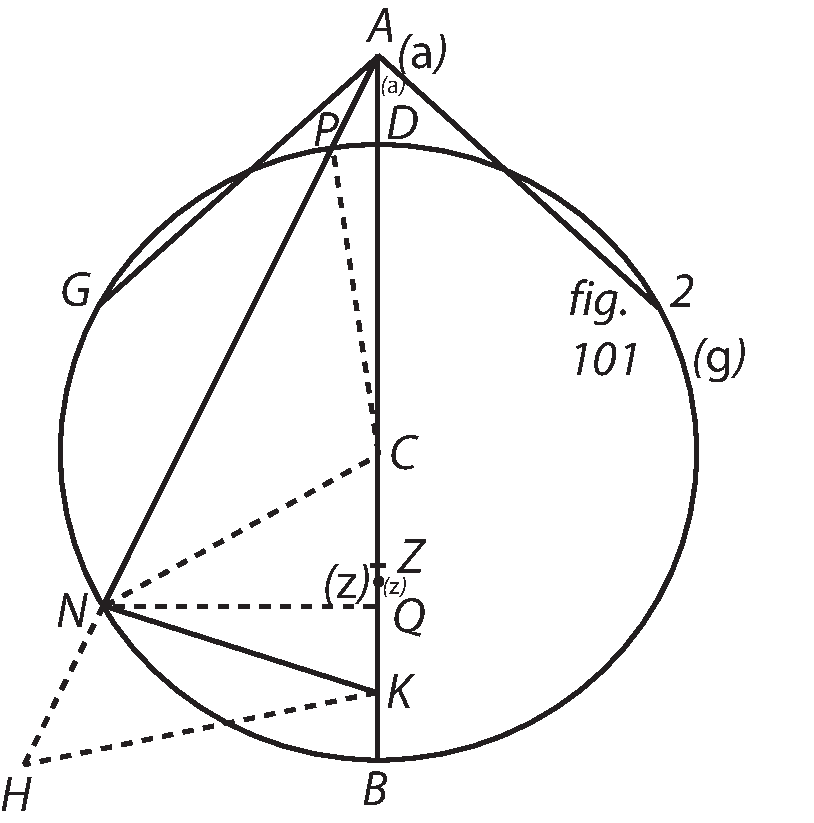
\includegraphics[trim = 0mm 0mm 0mm -5mm, clip,width=0.4\textwidth]{images/T8_Barrow-2.pdf}
\end{center}
\clearpage